\section{L'architettura U-Net}
% Una fra le tante architetture disponibili che possono essere utilizzate 
% per problemi di segmentazione semantica, è ad esempio l'architetture U-Net.
\label{section:U-Net}
U-Net è una rete neurale convoluzionale che si basa su un architettura 
cosiddetta \textit{Fully convolutional Network}  (rete completamente convoluzionale).
L'U-Net è un'architettura che ha guadagnato un grande popolarità 
grazie alle sue alte prestazioni nelle attività di segmentazione delle immagini. 
Introdotta nel 2015 da Olaf Ronneberger, Philipp Fischer e Thomas Brox nell'articolo 
"\textit{Convolutional Networks for Biomedical Image Segmentation}" \cite{ARTICOLO_ORIGINALE_UNET}, 
U-Net era stata originariamente pensata per affrontare problemi di segmentazione 
nel campo delle immagini biomediche. 
Ma grazie alla sua flessibilità ed efficacia, l'architettura ha trovato applicazione 
in numerosi altri settori.
U-Net è stata progettata principalmente per funzionare con dati di immagini in scala di grigi.
Ma può essere facilmente adattata per gestire immagini multicanale o anche volumi 3D.
Esistono molte varianti di questa architettura, che differiscono principalmente su parametri delle 
convoluzioni e dei polling. 
Esistono delle versioni che aumentano il numero degli strati o il numero di convoluzioni in 
ogni strato, migliorando la capacità della rete di apprendere rappresentazioni più complesse. 
Tuttavia, l'architettura originale è strutturata come segue:

\begin{figure}[H]
    \centering
    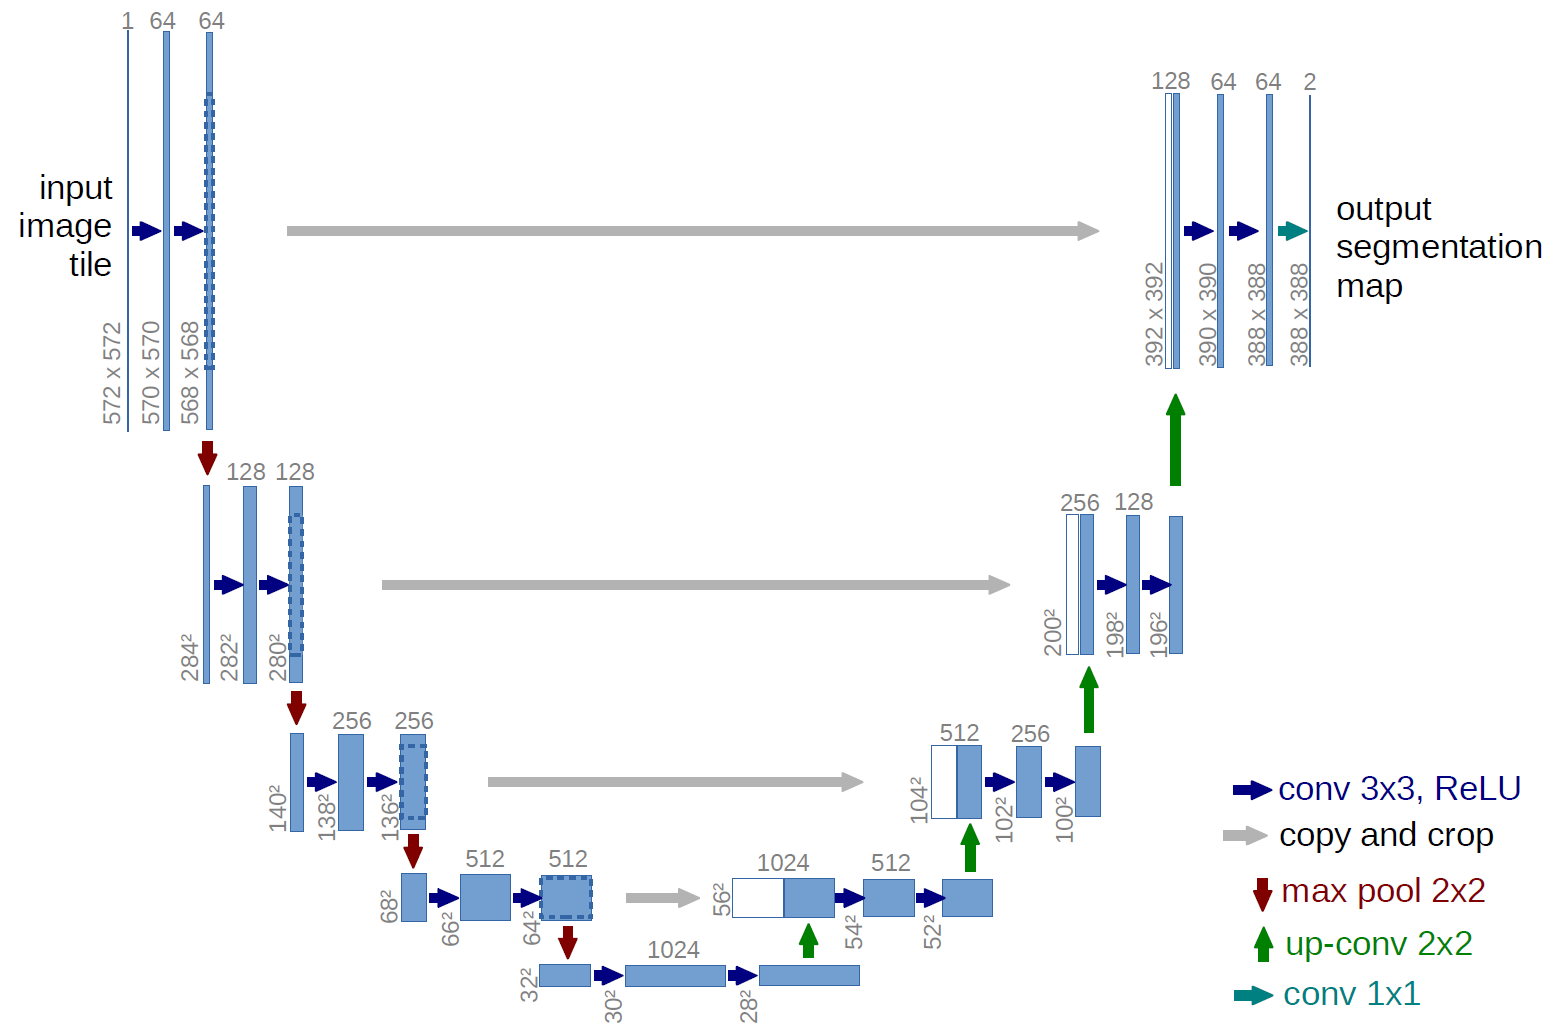
\includegraphics[width=0.8\textwidth]{Immagini/Generiche/UNET_LARGE.png}
    \caption{Rappresentazione dell'architettura U-Net \cite{ARTICOLO_ORIGINALE_UNET}.}
    \label{fig:UNET_ORIGINAL}
\end{figure}

%Una di queste variazioni è ad esempio la seguente struttura:

% \begin{figure}[H]
%     \centering
%     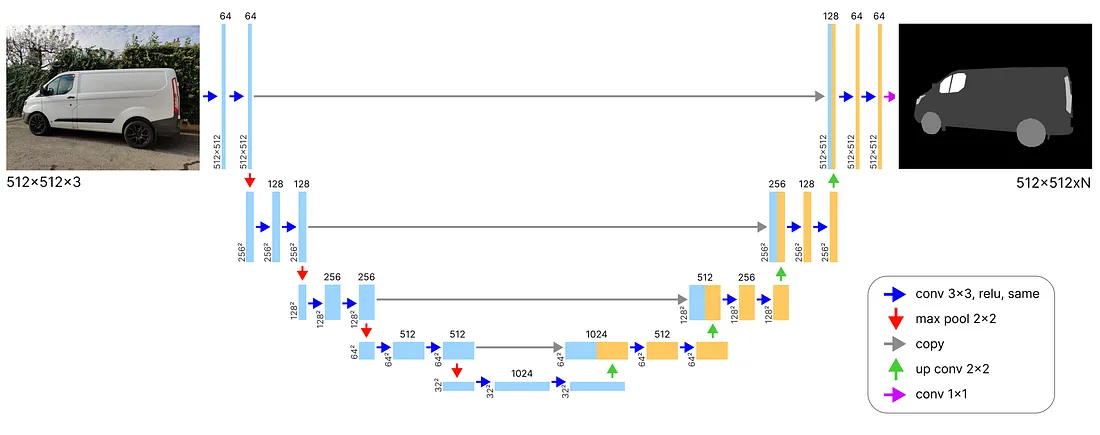
\includegraphics[width=1\textwidth]{Immagini/Generiche/UNET.png}
%     \caption{Rappresentazione dell'architettura U-Net \cite{Imagesegmentation_pulapakura}.}
%     \label{fig:UNET}
% \end{figure}

Come possiamo osservare dalla figura \ref{fig:UNET_ORIGINAL}, l'U-Net si basa su una 
struttura \textbf{encoder-decoder}, che caratterizza la sua forma ad "U" da cui prende il nome.
L'\textit{encoder} e il \textit{decoder} svolgono le seguenti funzioni:

\begin{itemize}
    \item L'\textbf{encoder} viene utilizzato per comprimere l'immagine di ingresso in 
    una rappresentazione dello spazio latente (uno spazio multidimensionale astratto 
    contenente valori caratteristici che non si possono interpretare direttamente, ma che sono  
    codificati in una rappresentazione interna significativa \cite{SPAZIO_LATENTE})
    attraverso convoluzioni e downsampling \cite{APSETTI_UNET}.

    \item Il \textbf{decoder} viene utilizzato per estrapolare la 
    rappresentazione latente in un'immagine segmentata, 
    attraverso convoluzioni e upsampling \cite{APSETTI_UNET}.
\end{itemize}

\subsection{skip connections}
Le lunghe frecce grigie che attraversano la "U" sono le \textbf{skip connections} (o connessioni di salto) 
e hanno due scopi principali:

\begin{itemize}
    \item Durante \textit{forward} dei dati, consentono al \textit{decoder} di accedere alle 
    informazioni dell'\textit{encoder}.

    \item Durante la \textit{backward}, agiscono come una "superstrada del gradiente" 
    (\textit{gradient superhighway}) per il flusso dei gradienti dal 
    \textit{decoder} all'\textit{encoder}.
\end{itemize}

\subsection{Up-Convolution}
Nella figura \ref{fig:UNET_ORIGINAL}, le frecce verdi rappresentano l'operazione 
di \textbf{Up-Convolution}.
L'\textit{up-convolution}, nota anche come deconvoluzione o convoluzione trasposta, 
è un metodo utilizzato per sovracampionare (upsample) le immagini e recuperare le 
informazioni spaziali.

\begin{figure}[H]
    \centering
    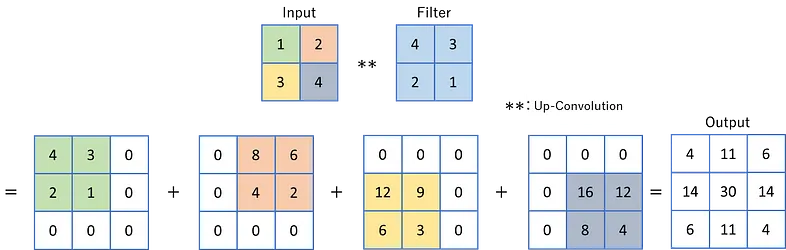
\includegraphics[width=0.76\textwidth]{Immagini/Generiche/up_conv.png}
    \caption{Rappresentazione dell'operazione di Up-Convolution \cite{APSETTI_UNET}.}
    \label{fig:Up-Convolution}
\end{figure}

\subsection{La funzione di attivazione nella convoluzione di uscita}
Nella convoluzione di uscita, la funzione di attivazione che segue la convoluzione dipende dal 
numero di classi che vogliamo distinguere.
Nei casi di \textit{Binary Segmentation} (ovvero quando dobbiamo distinguere due classi), 
tipicamente si utilizza la sigmoide, che restituisce dei valori tra 0 e 1.
Questi valori possono essere interpretati come delle probabilità. 

Mentre quando si hanno più di 2 classi, la funzione di attivazione che viene utilizza 
è la softmax, la quale opera sui canali di ogni pixel. Ridefinendo i valori di ogni singolo
canale del pixel come una distribuzione di probabilità.


\subsection{Output della rete}
\begin{multicols}{2}
    {Il risultato della rete è un'immagine composta da tanti canali, tanti 
    quanto sono le classi che vogliamo riconoscere.
    Pertanto, ogni canale del pixel rappresenta la probabilità di 
    associare al pixel la classe 
    rappresentata dal canale.
    Ad esempio, la figura qui a lato mostra il risultato della rete utilizzando 5 classi.}
    {
        \begin{figure}[H]
            \centering
            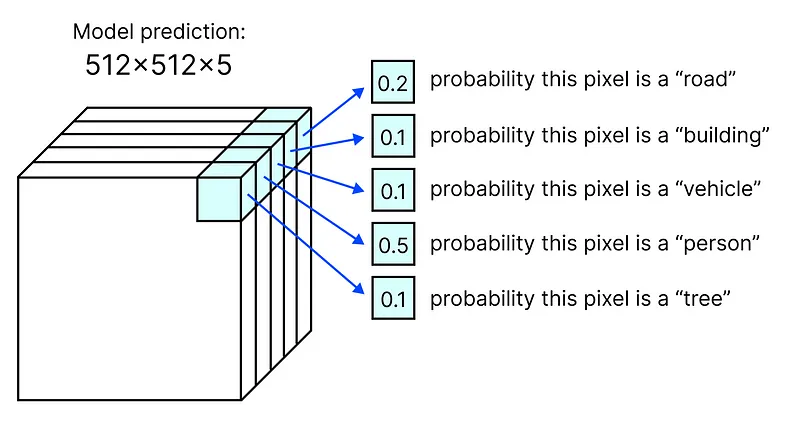
\includegraphics[width=0.52\textwidth]{Immagini/Generiche/softmax_UNET.png}
            \caption{Rappresentazione dell'output della U-net \cite{Imagesegmentation_pulapakura}.}
            \label{fig:UNET_OUTPUT}
        \end{figure}
    }
\end{multicols}






